{
  \newmdenv[tikzsetting={draw=black,fill=white,fill opacity=0.7, line width=4pt},backgroundcolor=none,leftmargin=0,rightmargin=0,innertopmargin=4pt,skipbelow=\baselineskip,%
  skipabove=\baselineskip]{TitleBoxWhatDoesMonadMean}

  \usebackgroundtemplate{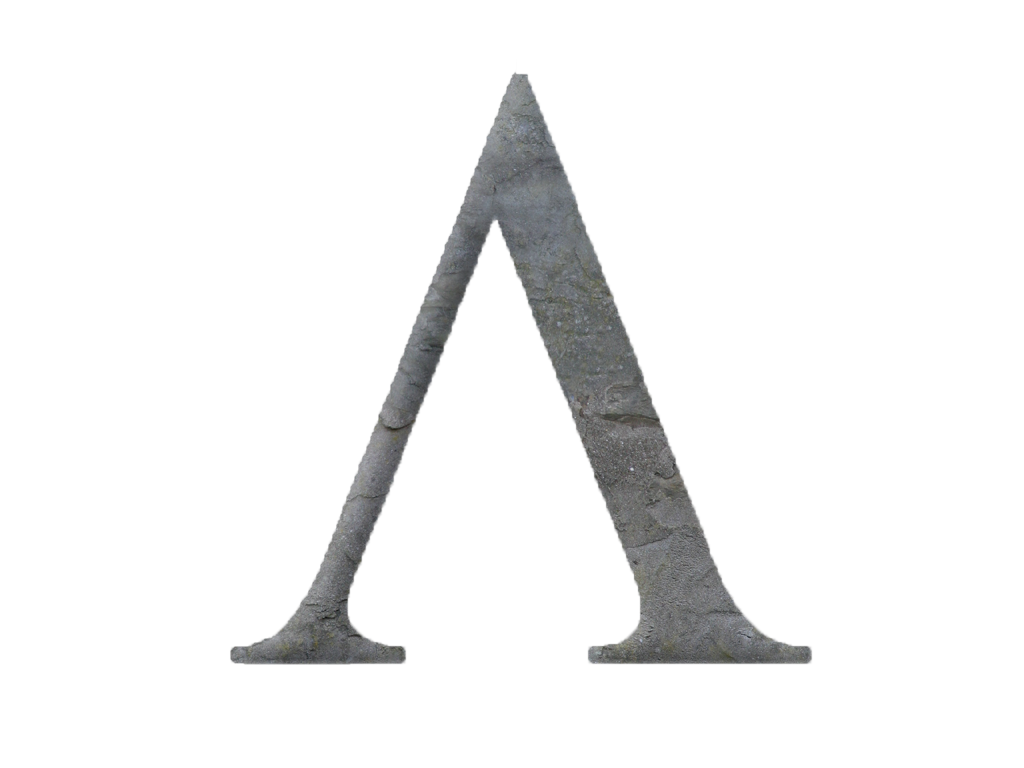
\includegraphics[width=1.0\paperwidth]{image/title-background.png}}

  \begin{frame}[plain] 
  \title{What Does Monad Mean?}
  
  \vspace{3em}

  \begin{TitleBoxWhatDoesMonadMean}
    \begin{center}
    {\Large \inserttitle}
    \end{center}
  \end{TitleBoxWhatDoesMonadMean}

  \end{frame}
}


\begin{frame}
\frametitle{What Does Monad Mean?}
\begin{block}{Well if you google it}
burritos, spacesuits or some shit like that
\end{block}
% wrong question
\end{frame}


\begin{frame}
\frametitle{What Does Monad Mean?}
\begin{block}{I want to do three things}
\begin{enumerate}
  \item establish the principles of abstraction and what is required to exploit them
  \item come to understand the relationship between monads and functional programming \emph{\tiny{(spoiler: there isn't one)}} \normalsize
  \item arm you with the skills to recognise common myths
\end{enumerate}
\end{block}
\end{frame}


\begin{frame}
\frametitle{Principles and Goals of Abstraction}
\begin{block}{Construct a constraint}
\begin{itemize}
  \item minimise the requirements to satisfy the constraint to increase instances
  \item maximise potential for deriving operations as a consequence of satisfying the constraint 
\end{itemize}
\end{block}
\end{frame}


\begin{frame}
\frametitle{Principles and Goals of Abstraction}
\begin{block}{Trade-off between the two}
\begin{itemize}
  \item stronger constraint
    \begin{itemize}
      \item fewer instances
      \item more derived operations
    \end{itemize}
  \item weaker constraint
    \begin{itemize}
      \item more instances
      \item fewer derived operations
    \end{itemize}
\end{itemize}
\end{block}
\end{frame}


\begin{frame}
\frametitle{Principles and Goals of Abstraction}
\begin{block}{The ultimate goal}
Avoid repetition of the same work
\end{block}
\end{frame}


\begin{frame}
\frametitle{Principles and Goals of Abstraction}
\begin{block}{Consequently}
A proposed abstraction that loses in both directions is a \emph{false economy} and must be efficiently discarded
\end{block}
\end{frame}


\begin{frame}
\frametitle{Monad}
\begin{block}{Monad is another abstraction}
\begin{itemize}
  \item not expressible in degenerate static type systems
  \item difficult to demonstrate without a static type system
\end{itemize}
\end{block}
\end{frame}


\begin{frame}[fragile]
\frametitle{Monad}
\begin{block}{So sorry, but I must use a practical programming language now}
\begin{lstlisting}[style=haskell,mathescape]
class Monad f where
  (=<<) :: (a -> f b) -> f a -> f b
  unit  :: x -> f x
\end{lstlisting}
\end{block}
\end{frame}


\begin{frame}[fragile]
\frametitle{Monad}
\begin{block}{This abstraction has many instances (values for \lstinline$f$)}
\begin{itemize}
  \item list
  \item continuations
  \item nullable values
  \item exception chaining
  \item state
  \item I/O actions
  \item argument threading
  \item logging
  \item \emph{hundreds more}
\end{itemize}
\end{block}
\end{frame}


\begin{frame}
\frametitle{Monad}
\begin{block}{This abstraction gives rise to many useful operations}
\begin{itemize}
  \item sequencing a list of effect values

        \lstinline$[f a] -> f [a]$
  \item replicating an effect a given number of times

        \lstinline$Int -> f a -> f [a]$
  \item \emph{bazillions more}
\end{itemize}
\end{block}
\end{frame}


\begin{frame}
\frametitle{Monad}
\begin{block}{We just saw}
\begin{itemize}
  \item<1> the monad abstraction expressed as a constraint
  \item<2> instances that satisfy the constraint
  \item<3> operations that are derived from the constraint
  \item<4> \textbf{Do not conflate these}
\end{itemize}
\end{block}
\end{frame}


\begin{frame}
\frametitle{Abstraction nomenclature}
\begin{block}{Other abstractions trade off along the two competing principles}
\begin{itemize}
  \item covariant functor
  \item applicative functor
  \item semigroupoid
  \item comonad
  \item profunctor
  \item monoid
  \item \emph{hundreds more}
\end{itemize}
\end{block}
\end{frame}


\begin{frame}
\frametitle{Now that we know this}
\begin{block}{We can do some mythbusting}
\begin{itemize}
  \item<1-> Monads are for side-effects
  \item<2-> Monads are for functional programming only
  \item<3-> Monads are for doing I/O
  \item<4-> Monads don't apply to my programming tasks
  \item<5-> I use Python, so monads won't help me as much
\end{itemize}
\visible<6->{
  \begin{tikzpicture}[remember picture,overlay]
  \coordinate (aa) at ($(a1)+(1,4.5)$);
  \node[right] at (aa) {
\includegraphics[height=3cm]{image/bullshizzles.png}};
  \end{tikzpicture}
}
\end{block}
\end{frame}


\begin{frame}
\frametitle{Bullshizzles}
\begin{block}{Perfidious Seduction}
You will be invited to believe these things. Decide wisely.
\end{block}
\end{frame}


\begin{frame}
\frametitle{Abstraction and Python}
\begin{block}{Python}
Python achieves abstraction using dynamic structural-typing\footnote{aka duck typing}
\end{block}
\end{frame}


\begin{frame}
\frametitle{Abstraction and Python}
\begin{block}{Further to this}
You will rarely see even the most fundamental abstractions in these systems
\end{block}
\end{frame}


\begin{frame}
\frametitle{Abstraction and Python}
\begin{block}{Certainly}
You will never see any non-trivial abstraction \tiny{\emph{(above those already mentioned)}}\normalsize
\end{block}
\end{frame}


\begin{frame}
\frametitle{Abstraction and Python}
\begin{center}
\huge{Why might this be?}
\end{center}
\normalsize
\end{frame}
